\documentclass[11pt]{beamer}
\usepackage[utf8]{vietnam}
\usepackage{lmodern}
\usetheme{Warsaw}
\usepackage[backend=biber]{biblatex}

\addbibresource{presentation.bib}

\newcommand{\eg}{\text{e.g.\ }}

\begin{document}
\author{Trần Hoàng Quân, Lê Hoàng Trọng Tín, Lê Mai Nguyên Thảo}
\title{Trust Negotiations}
\subtitle{Tìm hiểu khái niệm và một số hệ thống thực tế}
\logo{
\includegraphics[scale=.2]{img/fithcmuslogo.png}}
\institute{Trường Đại học Khoa học tự nhiên - ĐHQG HCM \\ Khoa Công nghệ Thông tin}
%\date{}
%\setbeamercovered{transparent}
\setbeamertemplate{navigation symbols}{}
\begin{frame}[plain]
\maketitle
\end{frame}

\begin{frame}
\frametitle{Nội dung}
\tableofcontents
\end{frame}

\section{Giới thiệu}
\begin{frame}{Giới thiệu}
Một ví dụ trong thế giới thực: Bạn đi siêu thị mua hàng và thanh toán bằng thẻ tín dụng.
\begin{enumerate}
\item Nhân viên thu ngân xác nhận thẻ của bạn hợp lệ (\eg kiểm tra format số thẻ, kiểm tra 4 số security code, kiểm tra thẻ có bị chỉnh sửa tẩy xóa, ..etc).
\item Nhân viên thu ngân yêu cầu chủ thẻ nhập PIN và nhập số tiền.
\item Nhân viên thu ngân in biên lai và đưa bạn kí.
\item Nhân viên xác nhận chữ kí của bạn giống chữ kí phía sau thẻ, vậy là đã thanh toán thành công.
\end{enumerate}
\end{frame}

\begin{frame}{Giới thiệu (cont.)}
Giao dịch trong ví dụ trên có sự trao đổi thông tin (credentials) giữa người mua và người bán, từ đó thiết lập sự tin tưởng rằng người mua có đủ điều kiện để mua đồ, và người bán có đủ điều kiện để bán.

Mục đích cuối cùng của Trust Negotiation:
\begin{itemize}
\item Thiết lập sự tin cậy (Trust Establishment) giữa các bên tham gia.
\item Dù trao đổi nhiều thông tin (credentials) với nhau, credentials phải được giữ an toàn.
\end{itemize}
\end{frame}

\section{Trust Negotiation}
\begin{frame}{Trust Establishment}
Trust Establishment: thiết lập sự tin cậy giữa những "người lạ" trong hệ thống mở:
\begin{itemize}
\item Client và Server không cùng security domain.
\item Quyết định cấp quyền truy cập dựa vào thuộc tính (attribute), không dựa vào danh tính (identity).
\begin{itemize}
\item \eg Quyền của client trong tổ chức, loại ngành nghề, chức vụ, ..etc
\end{itemize}
\end{itemize}
\end{frame}

\begin{frame}{Trust Negotiation}
Trust Negotiation: phuơng pháp tiếp cận bằng cách kiểm soát truy cập (access control) và xác thực (authentication), cho phép người yêu cầu tài nguyên (Resource Requesters) và nhà cung cấp (Providers) thiết lập sự tin cậy trong các hệ thống mở, dựa trên các thuộc tính (attributes) hơn là danh tính (identity).
\begin{itemize}
\item Trao đổi digital credentials giữa các bên một cách tuần tự.
\item Đầu tiên trao đổi credentials ít nhạy cảm, khi độ tin cậy tăng thì trao đổi credentials nhạy cảm hơn.
\end{itemize}
\end{frame}


\begin{frame}{Trust Negotiation (cont.)}
\begin{figure}[H]
\centering
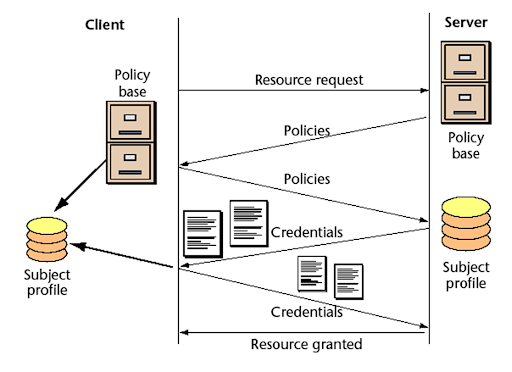
\includegraphics[scale=.4]{img/trust-simple.png}
\caption{Sơ đồ (đơn giản) của một mô hình Trust Negotiation}
\end{figure}
\end{frame}

\begin{frame}{Trust Negotiation (cont.) - Digital Credentials}
Digital Credentials: chứa các thuộc tính thông tin của người sở hữu, được cấp bởi một bên đáng tin cậy (thường là nhà cung cấp chứng thư số).
\begin{itemize}
\item Không thể làm giả.
\item Dễ xác thực.
\item Ký bằng PKI (public-key infrastructure, \eg chuẩn X.509 v3)
\end{itemize}
\end{frame}

\begin{frame}{Trust Negotiation (cont.) - Credential disclosure}
Credential disclosure policy (CDP):
\begin{itemize}
\item Điều kiện để một bên công bố các tài nguyên.
\item Bản thân credentials có thể có một số thông tin nhạy cảm, nên cũng được xem là một tài nguyên được bảo vệ.
\item Bản thân CDP cũng là một đối tượng được bảo vệ.
\end{itemize}
\end{frame}

\begin{frame}{Trust Negotiation (cont.) - Requirements}
Các yếu tố cần thiết cho một hệ thống Trust Management:
\begin{itemize}
\item Quyền sở hữu credential.
\item Tính hợp lệ của credential.
\item Khám phá credential chain.
\item Cơ chế bảo vệ quyền riêng tư.
\item Hỗ trợ các chiến thuật negotiate thay thế.
\begin{itemize}
\item \eg Tăng cường bảo mật, tối ưu tính toán, ..etc
\end{itemize}
\item Các chiến thuật negotiate nhanh.
\end{itemize}
\end{frame}

\begin{frame}{Trust Negotiation (cont.)}
Một số hệ thống trên thực tế:
\begin{itemize}
\item Keynote trust management system
\item Trust Establishment phát triển bởi Haifa Research lab
\begin{itemize}
\item Trust Policy Language (TPL)\cite{848442}
\end{itemize}
\item TrustBuilder
\item Unipro
\item Trust-X
\end{itemize}
\end{frame}

\section{Một số hệ thống trên thực tế}
\subsection{ATNAC}
\begin{frame}{ATNAC}
Adaptive Trust Negotiation and Access Control (ATNAC)\cite{10.1145/1063979.1064004} là kiến trúc access control cho các dịch vụ điện tử, kết hợp của hai hệ thống:
\begin{itemize}
\item TrustBuilder: Xác định cách thức tiết lộ thông tin nhạy cảm.
\item GAA-API: Kiểm soát truy cập một cách thích ứng.
\end{itemize}
\end{frame}

\begin{frame}{ATNAC (cont.) - Trust Builder}
TrustBuilder là hệ thống Trust Negotiation phát triển bởi Đại học Brigham Young (BYU) và Đại học Illinois Urbana-Champaign (UIUC):
\begin{itemize}
\item Dễ bị tấn công DoS (denial of service - từ chối dịch vụ).
\begin{itemize}
\item Số lượng lớn session Trust Negotiation được gởi lên server.
\item Server phải tính toán policy rất phức tạp.
\item Server phải tính toán credentials không liên quan hoặc không hợp lệ.
\end{itemize}
\item Các cuộc tấn công thường nhắm vào thông tin nhạy cảm.
\end{itemize}
\end{frame}

\begin{frame}{ATNAC (cont.) - GAA-API}
GAA-API: Generic Authorization and Access-control API
\begin{itemize}
\item Là middleware API
\item Fine-grained access control (FGAC - Kiểm soát truy cập chi tiết).
\item Phát hiện và phản hồi xâm nhập cấp ứng dụng.
\item Có thể tương tác với hệ thống phát hiện xâm nhập (Intrusion Detection System - IDS) để thích ứng với các điều kiện đe dọa mạng.
\item Không hỗ trợ Trust Negotiation.
\end{itemize}
\end{frame}

\begin{frame}{ATNAC (cont.) - GAA-API}
\begin{figure}
\centering
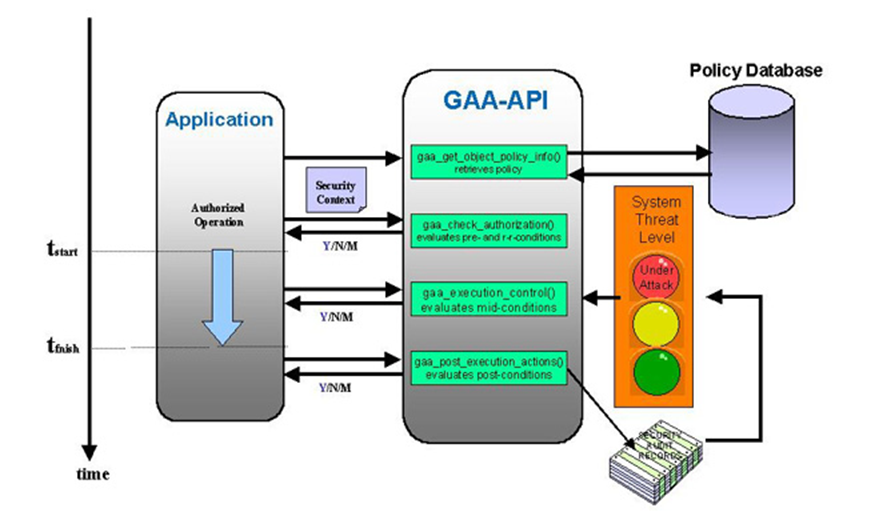
\includegraphics[scale=.5]{img/gaa-api.png}
\caption{Sơ đồ hệ thống với GAA-API middleware}
\label{fig:gaa_api}
\end{figure}
\end{frame}

\begin{frame}{ATNAC (cont.)}
Đặc điểm của ATNAC:
\begin{itemize}
\item Kết hợp hệ thống access control và Trust Negotiation để vá  khuyết điểm của mỗi hệ thống.
\item Hỗ trợ các chính sách thích ứng chi tiết (Fine-grained adaptive policies).
\item Giảm chi phí tính toán.
\end{itemize}
\end{frame}

\begin{frame}{ATNAC (cont.)}
Chức năng từng phần của ATNAC:
\begin{itemize}
\item GAA-API:
\begin{itemize}
\item Quy định access control policies cho tài nguyên, dịch vụ và hành động.
\item Các policies được thể hiện theo format EACL (Enhanced Access Control List).
\end{itemize}
\item TrustBuilder:
\begin{itemize}
\item Thi hành các policies bảo vệ thông tin nhạy cảm.
\item Dùng chứng chỉ số X.509 v3.
\item Dùng TPL policies.
\end{itemize}
\end{itemize}
\end{frame}

\begin{frame}{ATNAC (cont.) - framework}
\begin{figure}
\centering
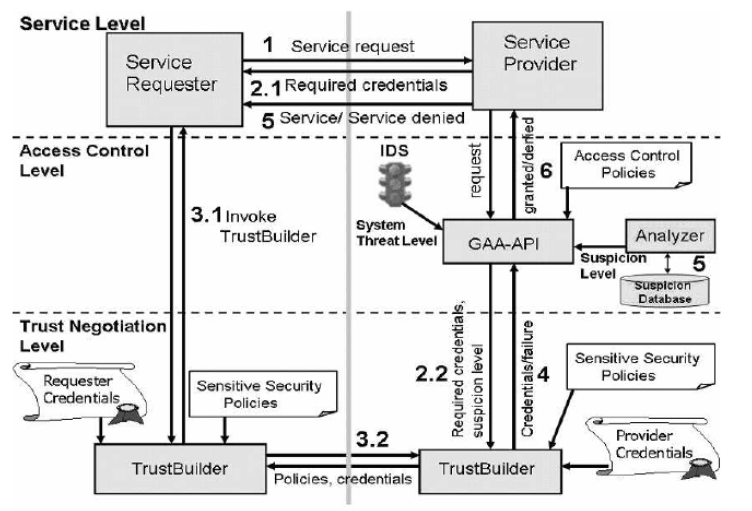
\includegraphics[scale=.5]{img/atnac.png}
\caption{Sơ đồ ATNAC framework}
\label{fig:atnac}
\end{figure}
\end{frame}

\begin{frame}{ATNAC (cont.) - Suspicion Level}
Mức nghi ngờ (Suspicion level) đánh giá khả năng một Requester đang thực hiện hành động không phù hợp. Mỗi Requester của một service có một Suspicion Level riêng biệt. Gồm 3 thành phần chính:
\begin{itemize}
\item $S_\text{DOS}$: Khả năng Requester đang thực hiện tấn công DoS.
\item $S_\text{IL}$: Rò rỉ thông tin (information leakage).
\item $S_\text{O}$: Các hành vi còn lại.
\end{itemize}
Suspicion Level tăng khi một sự kiện đáng nghi xảy ra, giảm khi một sự kiện (được cho là) tích cực xảy ra.
\end{frame}

\begin{frame}{ATNAC (cont.) - Cách hoạt động}
\begin{itemize}
\item Analyzer xác định các Requesters gởi một số lượng request tương đồng cao bất thường và tăng $S_\text{DOS}$.
\item Trong quá trình trust negotiation, credentials gởi bởi client phải trùng với credentials hệ thống yêu cầu, nếu không $S_\text{DOS} = 1$.
\item Nếu $S_\text{DOS}, S_\text{IL}$ hoặc $S_\text{O} > 0.9$, hệ thống sẽ dùng firewall chặn Requester.
\item Nếu $S_\text{IL} > \textit{một ngưỡng nhất định}$, TrustBuilder sẽ áp các chính sách nghiêm ngặt hơn với credentials, nhất là các credentials nhạy cảm.
\item Khi $S_\text{IL}$ tăng, GAA-API dùng các access control policies chặt chẽ hơn.
\end{itemize}
\end{frame}

\begin{frame}{ATNAC (cont.) - ví dụ}
\begin{columns}
\begin{column}{0.5\textwidth}
\begin{figure}
\centering
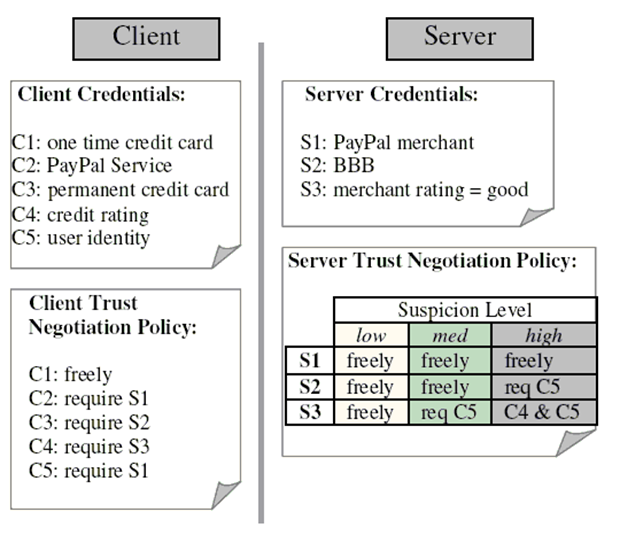
\includegraphics[scale=.4]{img/atnac-example-1.png}
\caption{Credentials và Policies của client và server}
\label{fig:atnac-1}
\end{figure}
\end{column}
\begin{column}{0.5\textwidth}
\begin{figure}
\centering
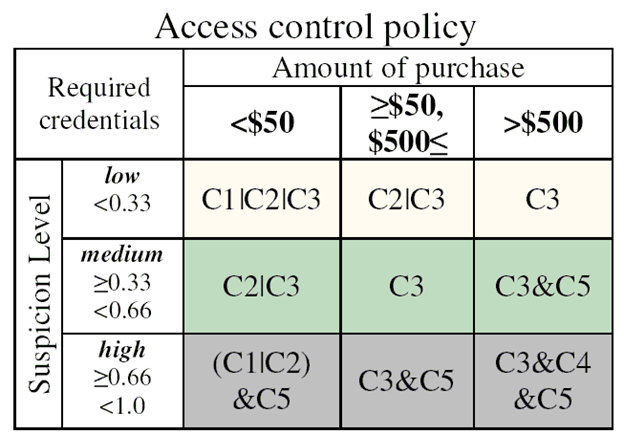
\includegraphics[scale=.4]{img/atnac-example-2.png}
\caption{Access control policy}
\label{fig:atnac-2}
\end{figure}
\end{column}
\end{columns}
\end{frame}

\subsection{Trust-X}
\begin{frame}{Trust-X}
Trust-X: P2P framework dành cho Trust Establishment\cite{10.1109/TKDE.2004.1318565}
\begin{itemize}
\item Hệ thống dựa trên XML
\item Thiết kế cho môi trường P2P.
\begin{itemize}
\item Mỗi bên chịu trách nhiệm tương đương trong quản lý thương lượng (negotiation management).
\item Bên nào cũng có thể là Requester hoặc Controller của một resource.
\end{itemize}
\item X-TNL: Ngôn ngữ đặc tả các certificate và policies dựa trên nền XML.
\end{itemize}
\end{frame}

\begin{frame}{Trust-X (cont.)}
\begin{itemize}
\item Certificates: có 2 loại:
\begin{itemize}
\item Credentials: Thể hiện đặc điểm của chủ sở hữu, được công nhận bởi CA (certificate authority).
\item Declarations: Chứa thông tin của chủ sở hữu, không cần được chứng nhận.
\end{itemize}
\item Trust tickets (X-TNL): dùng để tăng tốc quá trình negotiate khi đã được cấp quyền truy cập trong lần negotiate trước.
\item Negotiation tiến hành theo từng giai đoạn (phase):
\begin{itemize}
\item Introductory phase
\item Policy Evaluation phase
\item Certificate Exchange phase
\end{itemize}
\end{itemize}
\end{frame}

\begin{frame}{Trust-X (cont.) - X-TNL}
\begin{columns}
\begin{column}{.5\textwidth}
\begin{figure}
\centering
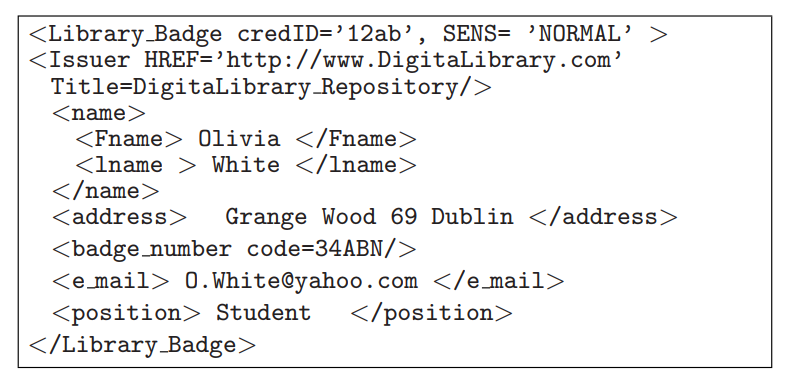
\includegraphics[scale=.3]{img/trustx-credential.PNG}
\caption{Credential XML}
\label{fig:trust_x_credential}
\end{figure}
\end{column}
\begin{column}{.5\textwidth}
\begin{figure}
\centering
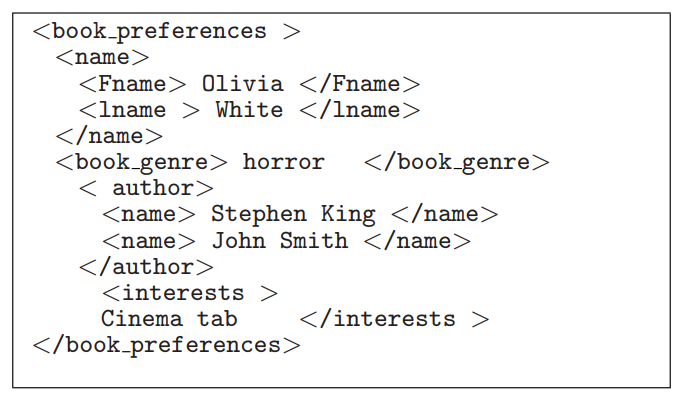
\includegraphics[scale=.3]{img/trustx-declaration.PNG}
\caption{Declaration XML}
\label{fig:trust_x_declaration}
\end{figure}
\end{column}
\end{columns}

\end{frame}


\begin{frame}{Trust-X (cont.) - Kiến trúc}
\begin{figure}
\centering
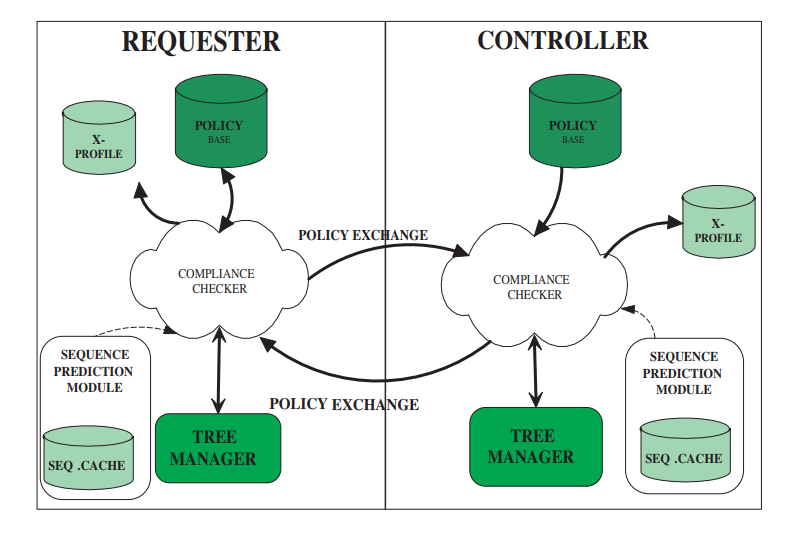
\includegraphics[scale=.5]{img/trust-x-architecture.PNG}
\caption{Kiến trúc Trust-X framework}
\label{fig:trust_x_architecture}
\end{figure}
\end{frame}

\begin{frame}{Trust-X (cont.) - Introduction phase}
Introduction phase:
\begin{itemize}
\item Bắt đầu khi Requester yêu cầu Controller cung cấp tài nguyên $\mathcal{R}$. 
\item Hai bên trao đổi với nhau bằng một số thông điệp ngắn.
\item Được quy định bởi các chính sách giới thiệu (introductory policies) của hai bên. Introductory policy được dùng để xác nhận các thuộc tính cần thiết cho các bước negotiate sau này.
\end{itemize}
\end{frame}

\begin{frame}{Trust-X (cont.) - Ví dụ Introduction phase}
Xét ví dụ một cửa hàng cho thuê xe. Alice muốn thuê một chiếc xe từ cửa hàng này và bắt đầu quá trình negotiate. Những điều kiện mà cửa hàng có thể yêu cầu trong introduction phase được biểu diễn bởi các introductory policies sau:
\begin{itemize}
\item Car\_Rental$_{p} \leftarrow $ Preferred\_Customer()
\item Car\_Rental$_{p} \leftarrow $ Car\_Preferences()
\end{itemize}
Policy đầu tiên kiểm tra khách hàng có \textit{preferred customer} credential thể hiện trước đó đã có giao dịch giữa hai bên. Policy thứ hai yêu cầu khách hàng gởi \texttt{car\_preferences} declaration để có thể chọn các loại xe phù hợp với yêu cầu của khách hàng.
\end{frame}

\begin{frame}{Trust-X (cont.) - Policy Evaluation phase}
Policy Evaludation phase:
\begin{itemize}
\item Client và server trao đổi các disclosure policies áp dụng cho các tài nguyên liên quan.
\item Policy Evaluation phase được thực hiện bởi Compliance Checker
\item Sử dụng cấu trúc cây Tree Manager để quản lí và cập nhật.
\item \textbf{Không certificate nào được công bố trong phase này}. Mục tiêu của phase là xác định chuỗi các certificate phù hợp với disclosure policy của cả server và client khi phát hành tài nguyên.
\end{itemize}
\end{frame}

\begin{frame}{Trust-X (cont.) - Certificate Exchange phase}
Certificate Exchange phase:
\begin{itemize}
\item Mỗi bên công bố certificate của mình theo thứ tự xác định trong phase trước. Bên còn lại xác thực certificate hợp lệ.
\item Nếu không có vấn đề, phase kết thúc và tài nguyên được phát hành.
\end{itemize}
\end{frame}

\begin{frame}{Trust-X (cont.) - Certificate Exchange phase}
\begin{figure}
\centering
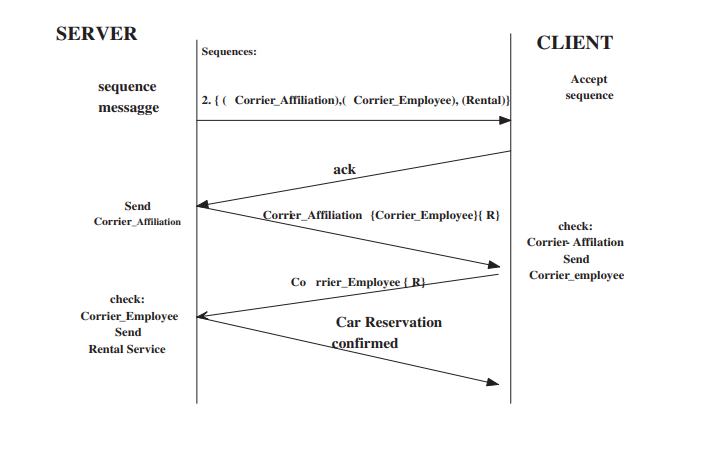
\includegraphics[scale=.5]{img/cert-exchange.PNG}
\caption{Ví dụ cho Certificate Exchange phase}
\label{fig:cert-exchange}
\end{figure}
\end{frame}

\begin{frame}{Trust-X (cont.) - Ví dụ}
Xem xét ví dụ về một công ty cho thuê xe (tạm gọi là công ty R):
\begin{itemize}
\item Nhân viên công ty \emph{Corrier} được miễn phí
\item Công ty R biết các nhân viên công ty \emph{Corrier} và có bản mềm bằng lái xe của mỗi người. Vì vậy, công ty R chỉ yêu cầu nhân viên trình thẻ công ty và một bản sao chứng minh thư hợp lệ để xác nhận đúng người.
\item Ngược lại, người lạ phải trả tiền để thuê xe và phải nộp bản mềm bằng lái \& thẻ tín dụng hợp lệ.
\end{itemize}
\end{frame}

\begin{frame}{Trust-X (cont.) - Ví dụ}
\begin{figure}
\centering
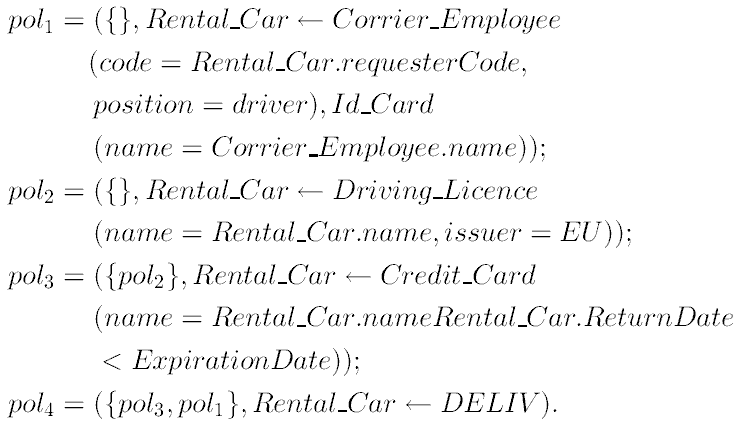
\includegraphics[scale=.5]{img/policy.png}
\caption{Hình thức hóa các policies trong ví dụ}
\label{fig:policy-formal}
\end{figure}
\end{frame}

\begin{frame}{Trust-X (cont.) - Negotiation}
\begin{figure}
\centering
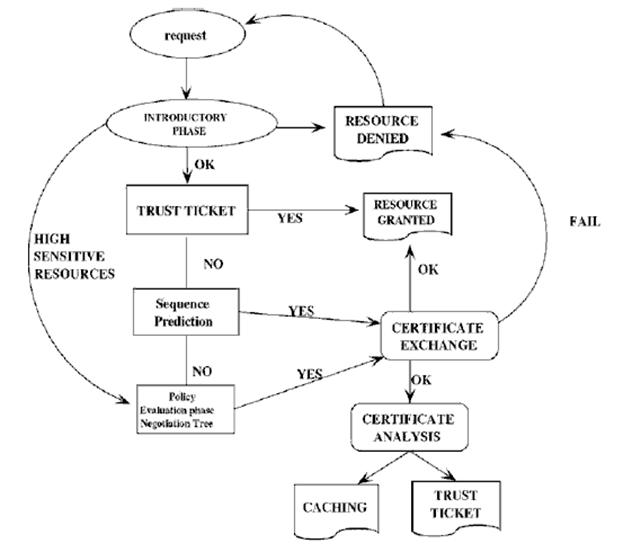
\includegraphics[scale=.5]{img/trustx-architecture.png}
\caption{Trust-X negotiation flow diagram}
\label{fig:trust-x-architecture}
\end{figure}
\end{frame}

\begin{frame}{Tổng kết}
ATNAC:
\begin{itemize}
\item Chống DoS
\item Tự động điều chỉnh security policies dựa trên Suspicion Level
\item Giám sát rò rỉ thông tin nhạy cảm.
\end{itemize}
Trust-X:
\begin{itemize}
\item P2P
\item Sử dụng X-TNL
\end{itemize}
\end{frame}

\begin{frame}[allowframebreaks]{Tài liệu}
\printbibliography
\end{frame}

\begin{frame}{}
\centering \Large
\emph{Fin}
\end{frame}

\end{document}